\subsection{Adaptation to Withheld Constraint Configurations}
\label{sec:v06-heldout}

\begin{figure*}[!t]
\centering
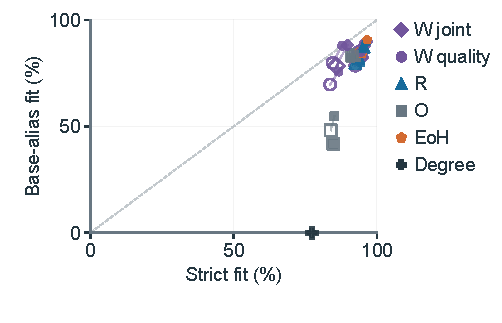
\includegraphics[width=.45\textwidth]{figures/heldout_strict_alias_movement_v06.pdf}\hfill
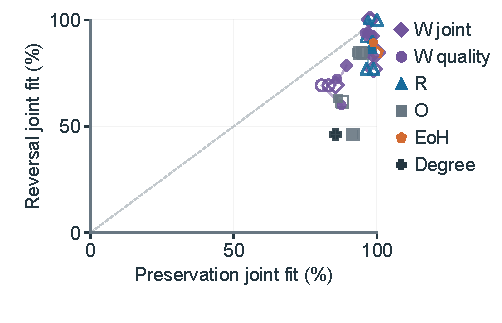
\includegraphics[width=.45\textwidth]{figures/heldout_pair_joint_movement_v06.pdf}
\Description{Strict versus base-alias scalar fit and strict-preservation versus strict-reversal joint correctness for the 21 predeclared main identities. Hollow points are original observations; solid points are the complete five-rename means, with thin connectors retaining movement.}
\caption{Frozen preference transfer: strict versus base-alias fit (left),
strict-preservation versus strict-reversal correctness (right). Hollow/solid
points denote original/five-rename means of all 21 predeclared identities;
coincident identities and renamings remain dependent.}
\label{fig:v06-heldout}
\end{figure*}

The mechanism TEST contains 24 source-disjoint public states and 48 newly
drawn contact endpoints forming 24 pairs. Contact generation retains TRAIN's
resource regimes and unit weights, but uses new seeds and withheld gaps
$0.25\!\to\!2$. Within a pair, the same contacts induce two conflict graphs.
All four W-joint rules omit the available gap coordinates and recompute
structural features from the current graph. No TEST preference label enters
their scoring. Certification occurs after the program
freeze and supplies evaluation targets only.

We evaluate 31 frozen identities and five prescribed identifier renamings.
Of 962 comparisons, 453 are strict (including 79
base-nine aliases) and 509 are exact ties. The 355 paired queries comprise
13 strict reversals, 83 strict preservations, 130 ties on both endpoints and
129 with one tied endpoint. All 190 quota shortfalls remain recorded.
Programs and selections freeze before evaluation certification; no TEST
outcome selects a winner.

Across four blocks, W joint attains mean original strict/base-alias fit of
91.94/81.96\%. Its strict advantage over W quality is 3.37 percentage points
(source-cluster 95\% interval: 2.04--4.72).
Joint-versus-quality comparisons include selection; intervals condition on
the frozen programs, not model-population effects. All four original demanded
feature quotients are acyclic. This evaluates scoped information repair and
actual scalar fit separately.

Both endpoints must satisfy their certified strict requirements for paired
correctness. Mean W joint reversal/preservation correctness is
82.69/95.48\% (Table~\ref{tab:v06-paired-adaptation}). These targets concern
configuration response, rather than arbitrary public-graph rankings.
Figure~\ref{fig:v06-heldout} retains every predeclared main
identity and its complete five-rename mean; no outcome selects plotted
programs. Renaming is a separate stress test, not an invariance guarantee.
The four EoH identities retain their seed origin and remain dependent.

\begin{table}[!t]
  \centering
  \caption{Ranking adaptation to gap $0.25\!\to\!2$ with identical contacts:
  all 13 reversal and 83 preservation requirements, original mapping.
  LLM rows average four dependent frozen outputs; Degree has one.
  EoH~\cite{liu2024eoh} retains a shared seed AST. Counts are output--requirement
  positions, not independent sources or scheduling gains.}
  \label{tab:v06-paired-adaptation}
  \setlength{\tabcolsep}{4pt}
  \begin{tabular}{lrr}
  \toprule
  Frozen cohort & Reversal (\%) & Preservation (\%) \\
  \midrule
  W joint & 82.69 (43/52) & 95.48 (317/332) \\
  W quality & 82.69 (43/52) & 89.76 (298/332) \\
  R quality & \textbf{86.54} (45/52) & 97.89 (325/332) \\
  O quality & 69.23 (36/52) & 92.17 (306/332) \\
  EoH-DSL & 84.62 (44/52) & \textbf{100.00} (332/332) \\
  Degree & 46.15 (6/13) & 85.54 (71/83) \\
  \bottomrule
  \end{tabular}
\end{table}


All 13,392 shared-kernel assignments complete with feasible incumbents.
The supporting report retains all 31 identities, full cohort contrasts,
renaming obstructions, rewards and measured costs; Discussion examines their
limits. These transfer measures characterize information repair; scheduling
quality is assessed separately.

